\section{Appendix: Building Layout}
\label{appendix:building}
\begin{figure}[H]
	\centering
	\textbf{Rooms and Capacities: Illini Union} \par\medskip
	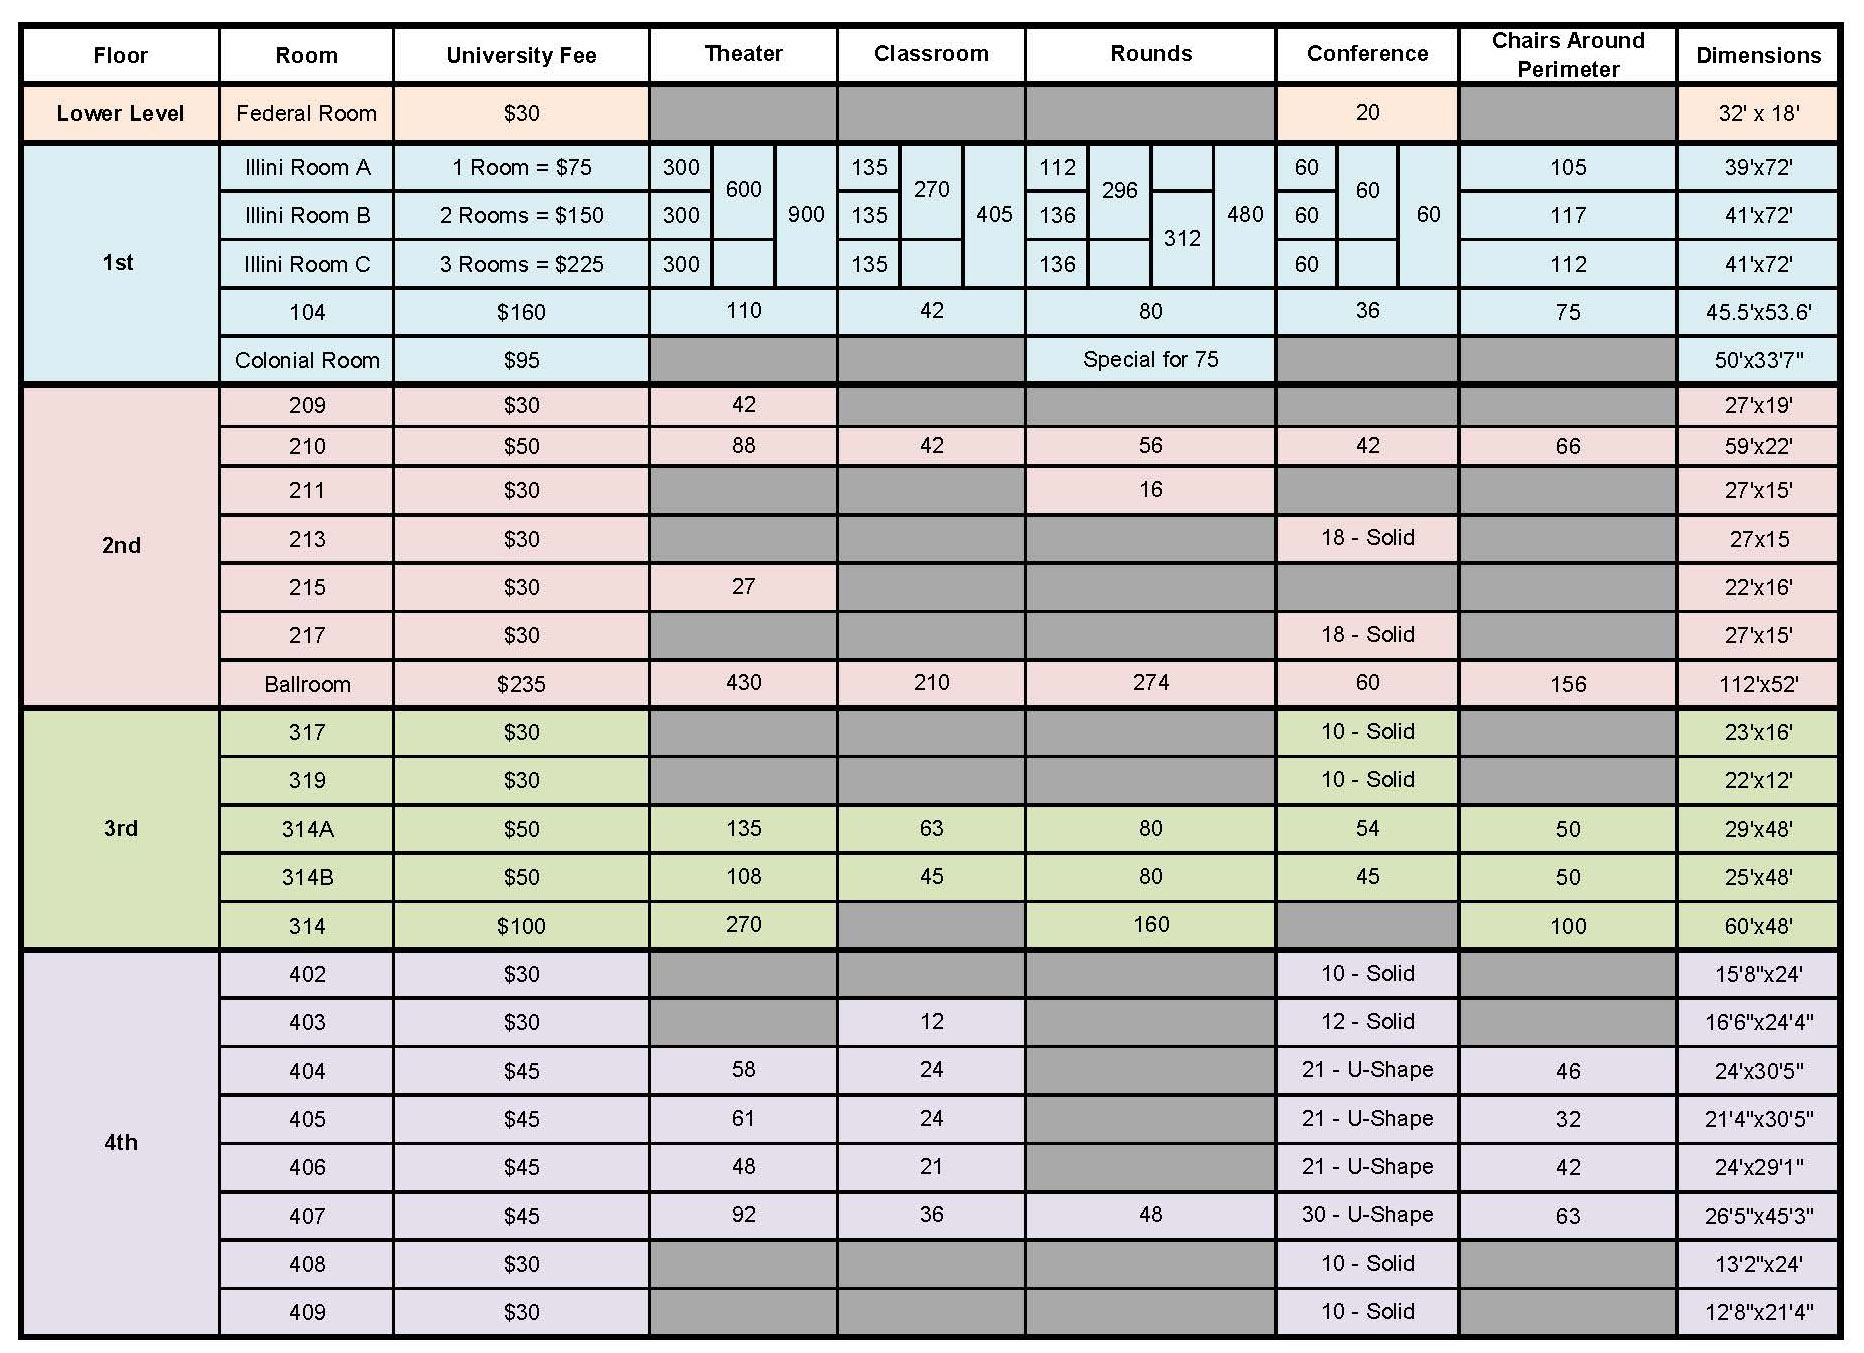
\includegraphics[width=\textwidth]{union-capacities.jpg}
\end{figure}

\newpage
{\centering\textbf{Floor Plans by Level: Illini Union} \par\medskip}
\begin{figure}[H]
	\centering
	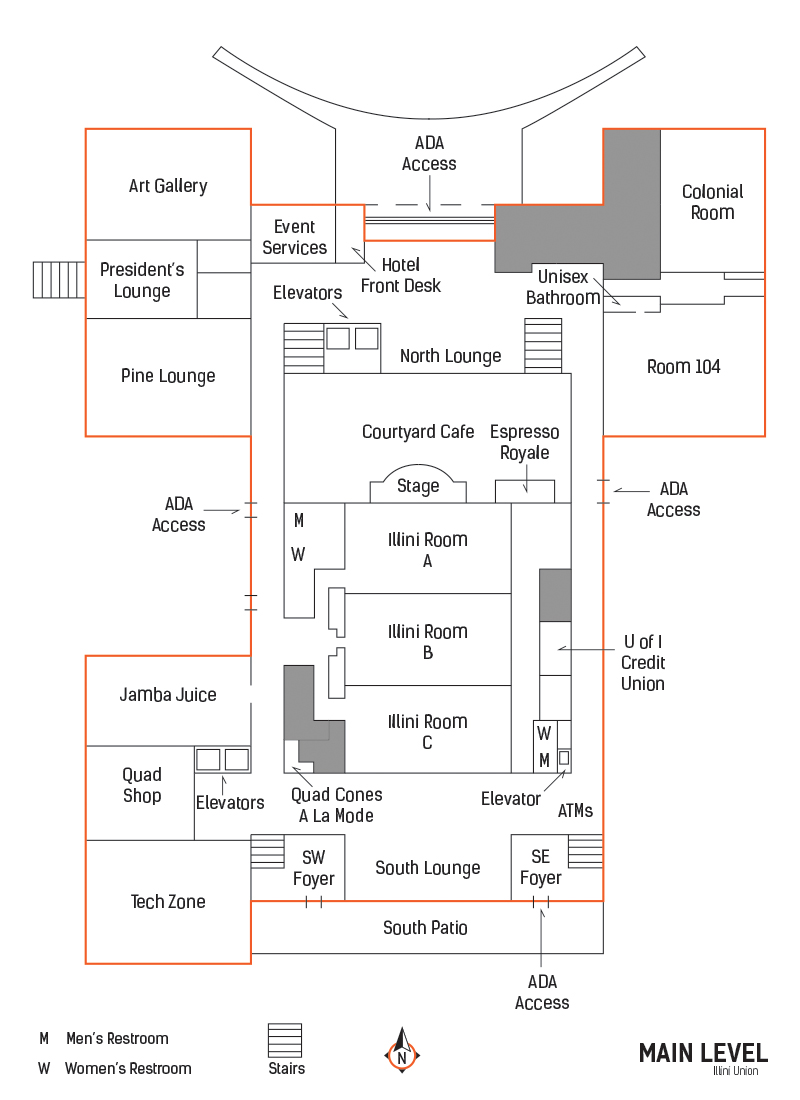
\includegraphics[width=0.75\textwidth]{unionlvl1.jpg}
	\caption{First Floor}
\end{figure}

\begin{figure}[H]
	\centering
	\begin{subfigure}{0.5\textwidth}
		\centering
		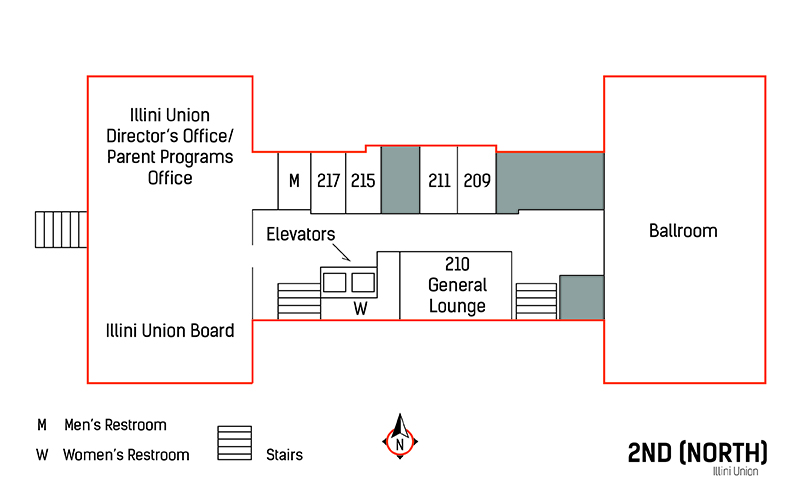
\includegraphics[width=0.9\linewidth]{unionlvl2.jpg}
		\subcaption{Second Floor - North Side}
	\end{subfigure}%
	\begin{subfigure}{0.5\textwidth}
		\centering
		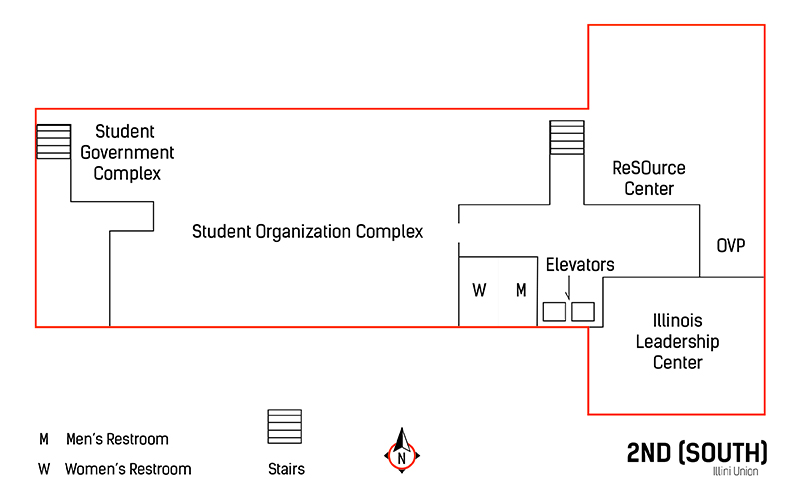
\includegraphics[width=0.9\linewidth]{unionlvl2s.jpg}
		\subcaption{Second Floor - South Side}
	\end{subfigure}
	\begin{subfigure}{0.5\textwidth}
		\centering
		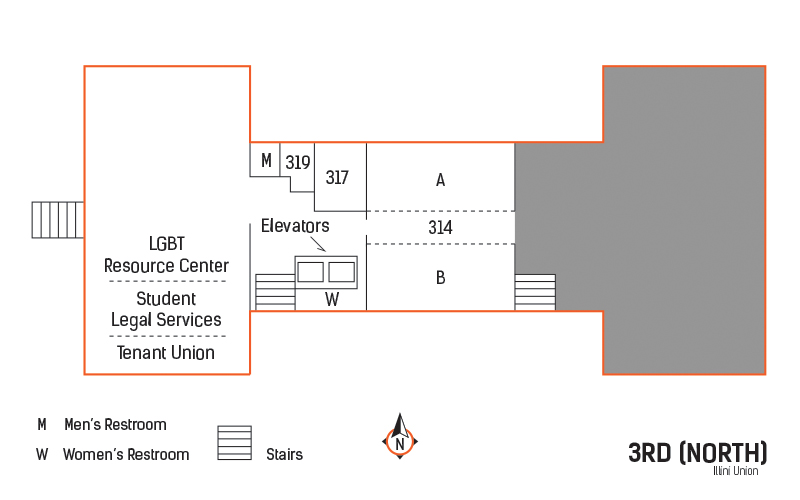
\includegraphics[width=0.9\linewidth]{unionlvl3.jpg}
		\subcaption{Third Floor}
	\end{subfigure}%
	\begin{subfigure}{0.5\textwidth}
		\centering
		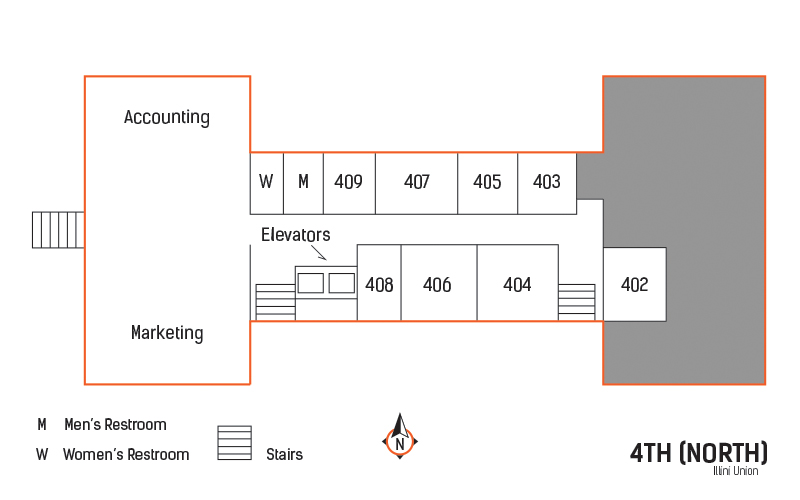
\includegraphics[width=0.9\linewidth]{unionlvl4.jpg}
		\subcaption{Fourth Floor}
	\end{subfigure}		
\end{figure}

\begin{figure}
	\centering
	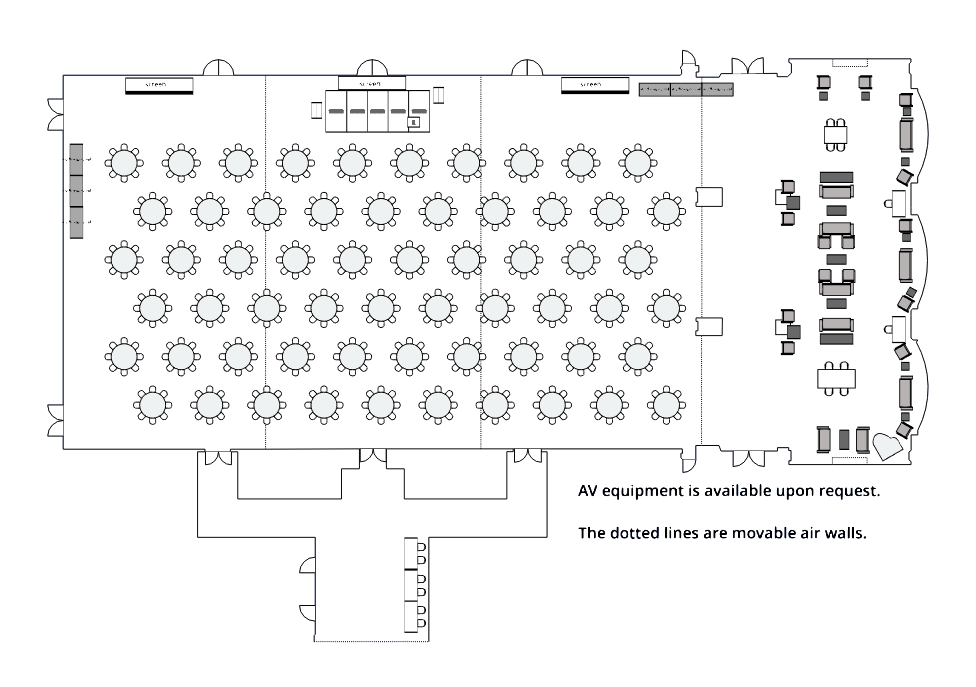
\includegraphics[width=0.8\textwidth]{union-banquet.png}
	\caption{Illini Rooms Banquet Space}
\end{figure}

\begin{figure}
	\centering
	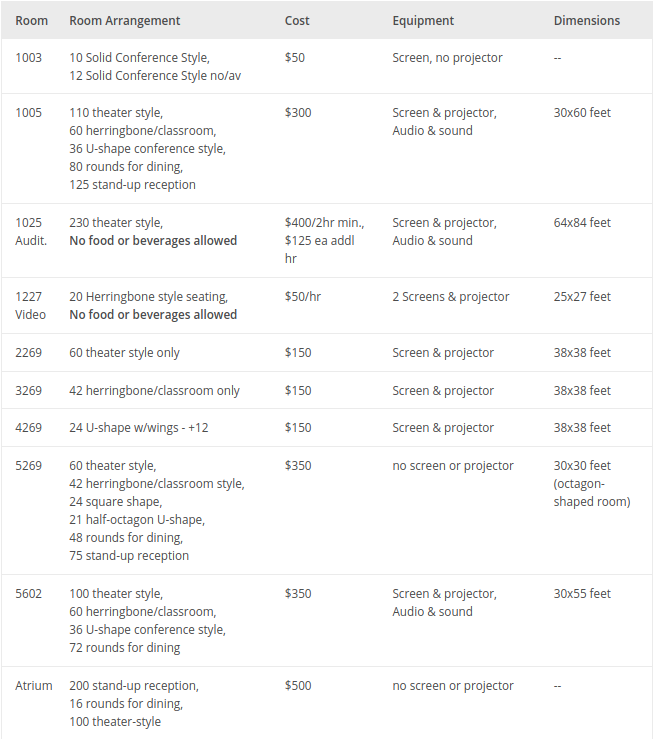
\includegraphics[width=\textwidth]{beckman-room-info.png}
	\caption{Information about the room capacities of Beckman Institute}
\end{figure}

\vspace{1cm}
\begin{figure}[H]
	\centering
	\textbf{I Hotel Floor Plan} \par\medskip
	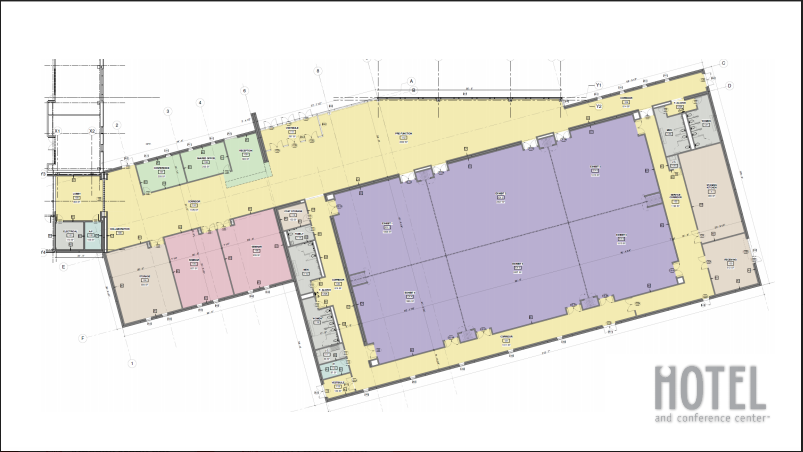
\includegraphics[width=\textwidth]{expanded-ihotel.png}
	\caption{Conference space for the expanded I Hotel.}
\end{figure}
\begin{figure}[H]
	\centering
	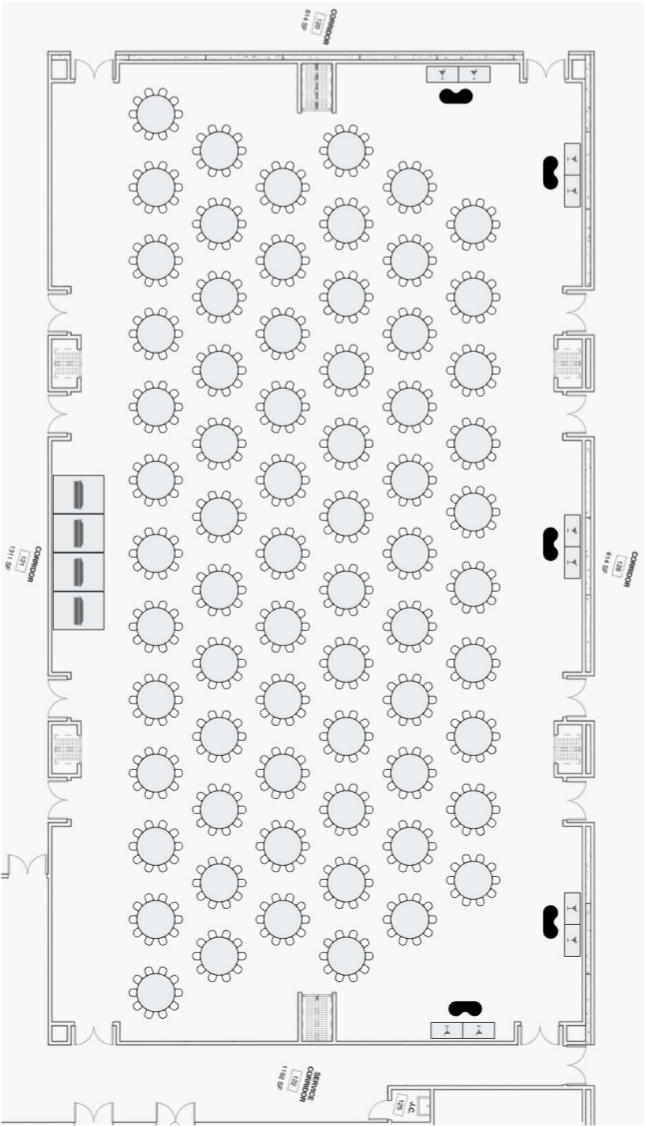
\includegraphics[angle=90, width=\textwidth]{ihotel-rounds.png}
	\caption{Seating for 690 in rounds at the I Hotel.}
\end{figure}
% 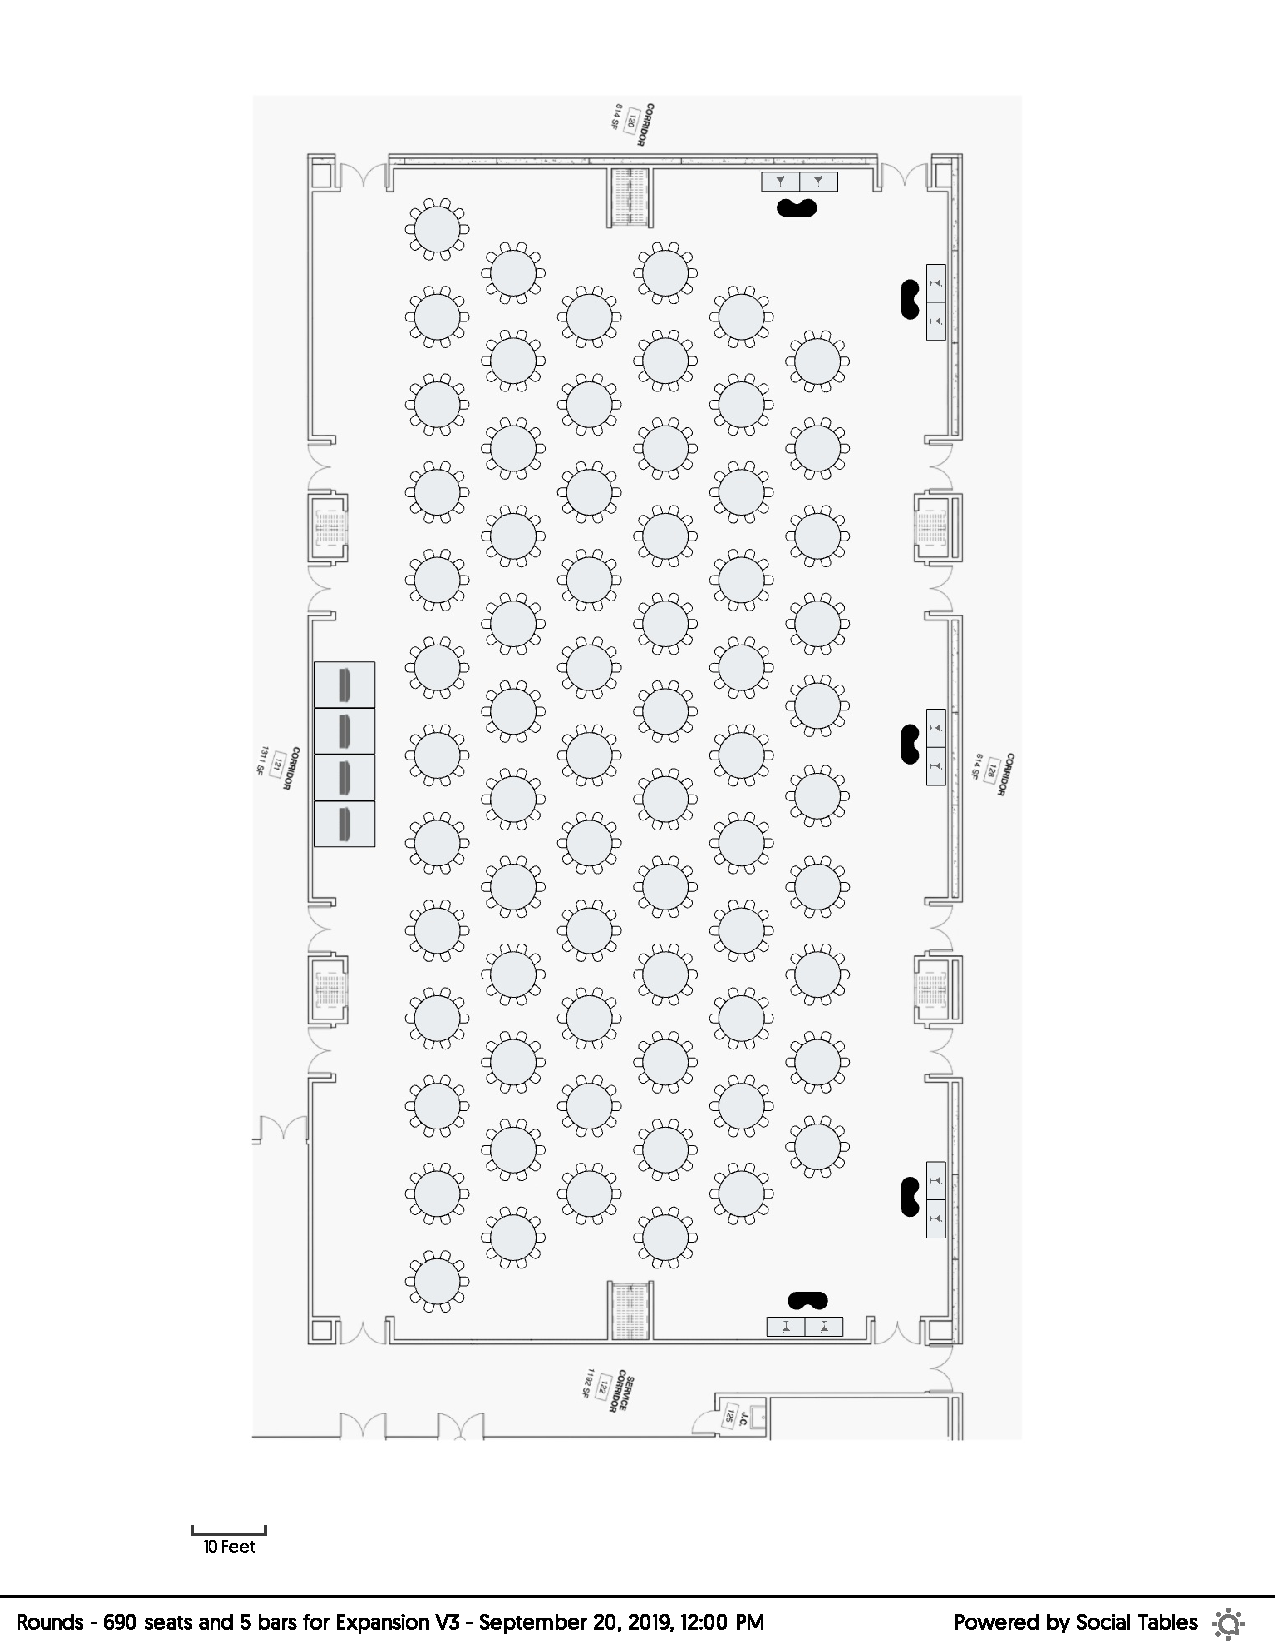
\includepdf[pages=1]{./documents/ihotel-banquet.pdf}
